\documentclass[12pt,spanish]{article}
\usepackage[utf8]{inputenc}
\usepackage{babel}
\usepackage{listings}
\usepackage{mathpazo}
\usepackage{enumitem}
\usepackage{courier}
\usepackage{textcomp}
\usepackage{xcolor}
\usepackage{parskip}
\usepackage{fullpage}

\newcommand{\onelinerule}{\rule[2.3ex]{0pt}{0pt}}
\newcommand{\twolinerule}{\rule[6.2ex]{0pt}{0pt}}
\newcommand{\respuesta}{\framebox[\textwidth]{\twolinerule}}
\newcommand{\nombre}{%
  \begin{tikzpicture}[xscale=.4,yscale=.7]
    \draw (0, 0) rectangle (22, 1);
  \end{tikzpicture}%
}
%\newcommand{\rol}   {\framebox[0.3\textwidth]{\onelinerule}}
\newcommand{\rol}{%
  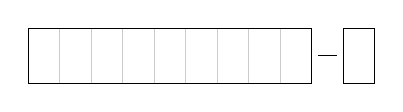
\begin{tikzpicture}[xscale=.4,yscale=.7]
    \draw[gray!40] ( 0, 0) grid      ( 9, 1);
    \draw          ( 0, 0) rectangle ( 9, 1);
    \draw          (10, 0) rectangle (11, 1);
    \draw (9 + .2, .5) -- (10 - .2, .5);
  \end{tikzpicture}%
}
\newcommand{\li}{\lstinline}
\providecommand{\pond}[1]{[{\small\textbf{#1\%}}]}

\lstdefinelanguage{py}{%
  classoffset=0,%
    morekeywords={%
      False,class,finally,is,return,None,continue,for,lambda,try,%
      True,def,from,nonlocal,while,and,del,global,not,with,print,%
      as,elif,if,or,yield,assert,else,import,pass,break,except,in,raise},%
    keywordstyle=\color{black!80}\bfseries,%
  classoffset=1,
    morekeywords={int,float,str,abs,len,raw_input,exit,range,min,max,%
      set,dict,tuple,list,bool,complex,round,sum,all,any,zip,map,filter,%
      sorted,reversed,dir,file,frozenset,open,%
      array,zeros,ones,arange,linspace,eye,diag,dot},
    keywordstyle=\color{black!50}\bfseries,%
  classoffset=0,%
  sensitive=true,%
  morecomment=[l]\#,%
  morestring=[b]',%
  morestring=[b]",%
  stringstyle=\em,%
}

\lstdefinelanguage{testcase}{%
  moredelim=[is][\bfseries]{`}{`},%
  backgroundcolor=\color{gray!20},%
}

\lstdefinelanguage{file}{%
  frame=single,%
}

\lstset{language=py}
\lstset{basicstyle=\ttfamily}
\lstset{columns=fixed}
\lstset{upquote=true}
\lstset{showstringspaces=false}
\lstset{rangeprefix=\#\ }
\lstset{includerangemarker=false}

\newlist{certamen}{enumerate}{1}
\setlist[certamen]{%
  label=\arabic*.,
  font=\LARGE\bfseries,%
  labelindent=-.5in,%
  leftmargin=0pt,%
  labelsep=1em%
}



\begin{document}
  \thispagestyle{empty}
  \section*{Miércoles 29 de agosto}
  Un analista financiero desea estudiar el comportamiento
  del precio del dólar de los últimos días.
  Para esto, le encargará a usted (y a su equipo)
  el desarrollo de un programa que le faciliten su tarea.

  El programa debe comenzar preguntando
  cuántos precios serán ingresados,
  y a continuación debe preguntar esos precios.

  \begin{enumerate}[leftmargin=0pt,start=0]

    \item
      Escriba el programa que pida al usuario ingresar los datos.

    \item
      Haga que su programa al final muestre
      cuál fue el promedio de los precios.
      ¿Cómo lo haría para que el precio sea mostrado
      siempre con una sola cifra decimal?

    \item
      Haga que su programa al final muestre
      cuántas veces el precio fue mayor que 490.

    \item
      Haga que su programa al final muestre
      la cantidad de alzas;
      es decir, cuántas veces el precio fue mayor
      al del día anterior.

      Si no hubo ninguna alza,
      el programa debe mostrar el mensaje
      \texttt{No hubo alzas}.

    \item
      Modifique su programa para que al final muestre
      cuál fue el precio más alto.

    \item
      Modifique su programa para que al final muestre
      cuál fue la mayor de las alzas.
      Si no hubo alzas, no debe mostrar nada.

  \end{enumerate}

  El siguiente es un ejemplo de cómo debería verse el programa terminado:

  \begin{minipage}[t]{0.6\textwidth}
    \lstinputlisting[language=testcase,frame=single]{entrada.txt}
  \end{minipage}

\end{document}

